\documentclass[
draft=false,
toc=graduated,
listof=totoc,
headsepline=true,
]%
{scrartcl}
\usepackage[utf8]{inputenc}
\usepackage[british]{babel}
\usepackage[babel, english=british]{csquotes}
\usepackage[T1]{fontenc}
\usepackage{mathpazo}
\usepackage[backend=biber,style=authoryear]{biblatex}
\ExecuteBibliographyOptions{
	bibwarn=true,
	bibencoding=utf8,
	maxbibnames=99,
    block=none,
	isbn=false,
	url=true,
	doi=true,
	eprint=true,
}
\setlength{\bibitemsep}{1em}
% References
\addbibresource{./references/references.bib}
\setcounter{tocdepth}{2}
\setcounter{secnumdepth}{3}
\usepackage[noenc, safe]{tipa}
\usepackage[]{hyperref}
\hypersetup{
	pdftitle={Documentation -- ParseEval in R},
	pdfauthor={Bastian Auris},	
	pdfcreator={Bastian Auris},
	pdfstartpage=1,
	pdfdisplaydoctitle=false,
	draft=false,
	colorlinks=false,
	linktoc=all,
}
\usepackage{graphicx}
\usepackage{multirow}
\usepackage{amsmath}
\usepackage{textcomp}
\usepackage{listings}
\lstset{
language=R,
basicstyle=\scriptsize\ttfamily,
commentstyle=\ttfamily\color{gray},
numbers=left,
numberstyle=\ttfamily\color{gray}\footnotesize,
stepnumber=1,
numbersep=5pt,
backgroundcolor=\color{white},
showspaces=false,
showstringspaces=false,
showtabs=false,
frame=single,
tabsize=2,
captionpos=b,
breaklines=true,
breakatwhitespace=false,
title=\lstname,
escapeinside={},
keywordstyle={},
morekeywords={}
}
\usepackage{tikz}
\usetikzlibrary{calc,arrows,intersections,shapes,positioning,patterns}
% docoment details
\title{ParseEval\footnote{\emph{ParseEval} is the name of the original \texttt{MATLAB} implementation introduced by \textcite{Shaw2009}. Since this is only an implementation of a similar functionality on a different platform i decided to keep it for practical reasons.} in \texttt{R}}
\subtitle{Documentation \& Reference}
\author{Bastian Auris}
\date{18th March 2013}
% custom
\newcommand{\HRule}{\rule{\linewidth}{0.5mm}}
\setcapindent{1em}
\setkomafont{captionlabel}{\sffamily\bfseries\small}

\begin{document}
\maketitle
\begin{abstract}
ParseEval is a function for assessing certain aspects of articulatory data in phonetic research. It is intended to be used to evaluate the fit between measurements taken from experimental data and measurements taken from simulated data generated under different syllable parses.\\
The purpose of this document is twofold. First off to act as a reference for using the ParseEval function and secondly to provide a hands-on guide (including a walk-through of example parses, etc.) to the possibilities when working with ParseEval in \texttt{R}~\footnote{\fullcite{Rcite}}. (This documentation assumes a basic level of familiarity with \texttt{R}.)

The ParseEval function on the other hand should be working with any recent version of \texttt{R} (\texttt{R} version $\geq$ 2.14). Although it is recommended to stay up-to-date on your \texttt{R}-installation and any additional packages you might be using.
Furthermore for the basic use of ParseEval it is \emph{not} required to have any additional packages installed; a basic, working install of \texttt{R} should be sufficient to produce results.

Although when it comes to plotting diagnostics (see section~\ref{subsec:latt}), it is preferred to utilize the \texttt{lattice} framework and the \texttt{gridExtra} package. In those cases it may be required to install additional packages. How to get this worked out is included in the description.\\
Skip to section~\ref{sec:guide} for the \enquote{User Guide}. If you feel comfortable enough to get in the middle of things right away, follow this link to the~\nameref{sec:qsg}.
\end{abstract}
\pagebreak
\tableofcontents
\listoffigures
\listoftables
\pagebreak
\section{Introduction}
\label{sec:intro}
\subsection{License}
Copyright \textcopyright{} 2013 Bastian Auris. This documentation is licensed under the Creative Commons Attribution-ShareAlike 3.0 Unported License.\par%
To view a copy of this license, visit \url{http://creativecommons.org/licenses/by-sa/3.0/} or send a letter to Creative Commons, 444 Castro Street, Suite 900, Mountain View, California, 94041, USA.
\subsection{Feedback}
Please use the ParseEval project page on GitHub to report bugs and submit feature requests\footnote{\url{https://github.com/phncgn-ba/parseeval\_in\_R}}. Before making a feature request, please ensure that you have thoroughly studied this manual. If you do not want to report a bug or request a feature but are simply in need of assistance, you might want to consider doing a web-search\footnote{e.g., via \href{https:\\www.google.com}{Google}}, visit Stack Overflow\footnote{\url{http://stackoverflow.com/questions/tagged/r}} or posting your question on a relevant newsgroup.
\subsection{Contributing}
Contributing to any part of the project is strongly encouraged. Contributions could range from proposed changes/improvements regarding the source-code, to work on the documentation (e.g. translating it), to being willing to share phonetic data for (reproducible) examples to be added to this document in future releases.
\subsection{Acknowledgements}
I would like to thank Jason A. Shaw, whose publications \parencite{Shaw2009,Shaw2011} inspired my work on ParseEval in \texttt{R}. He also provided me with the original \texttt{MATLAB} script and an extensive documentation accompanying it (on which I am going to draw on in parts during the course of this documentation). Moreover his helpful suggestions during the early stages of this project were essential in getting things rolling.\par
Furthermore I would like to thank \href{http://phonetik.phil-fak.uni-koeln.de/21.html}{Doris Mücke}, who supervised my BA thesis, which resulted in ParseEval for \texttt{R}.\par
Thanks to \href{http://phonetik.phil-fak.uni-koeln.de/143.html}{Anne Hermes} and \href{http://phonetik.phil-fak.uni-koeln.de/130.html}{Martine Grice}, for providing me with the Italian corpus-data that was analysed as part of the BA thesis (additionally used for the examples in the Quick start guide) and for sharing their phonetic insight on Italian on numerous occasions whenever questions arose.\par
\subsection{Prerequisites}
This section provides an overview of all resources required to achieve basic results running ParseEval in \texttt{R}. In case you find yourself struggling with \texttt{R} I would like to recommend the following:
\begin{description}
\item[Impatient R] click on the link to $\rightarrow$ \href{http://www.burns-stat.com/documents/tutorials/impatient-r/}{Impatient-R} which is a brief yet insightful intro to working with \texttt{R}.
\item[The R Inferno] excellent, (somewhat) humorous, book-sized guide $\rightarrow$ \href{http://www.burns-stat.com/documents/books/the-r-inferno/}{The R Inferno}. To quote the author:\enquote{If you are using R and you think you're in hell, this is a map for you.}.\\
This book aspires to be your guide while you venture through \texttt{R}, adapting Dante Alighieri's famous work, \enquote{Divine Comedy}.
\end{description}
Onto the requirements\dots{}
\subsubsection*{Requirements}
\begin{description}
\item[\texttt{R} software:] first and foremost you need to be able to access a running installation of the \texttt{R} software. You can download \texttt{R} from \url{http://www.r-project.org/} for the operating system of your choice. This website also offers extensive manuals for \texttt{R}, FAQ's and HOWTO's.\\%
Basic introduction to working with \texttt{R} cannot be covered by this documentation, but even if you have never seen or used \texttt{R}, the resources available on the website above should get you started.
\item[ParseEval (function):] Get the latest version of the ParseEval function (and possibly this documentation) from the ParseEval project-page on Github.
\end{description}
\newpage
\section{User Guide}
\label{sec:guide}
The following sections try to mimic the documents that one usually finds accompanying \texttt{R} packages. Although at this point in time ParseEval is not part a package, this might change in the future. The following sections are taken from Jason A. Shaw's original documentation of the MATLAB script, and adjusted for the purpose of this document.
\subsection{Description}
\begin{flushleft}
\begin{scriptsize}
(from Jason Shaw's original documentation)
\end{scriptsize}
\end{flushleft}
ParseEval is the \texttt{R} implementation of a MATLAB script that evaluates the fit between measurements taken from experimental data and measurements taken from simulated data generated under different syllable parses. A description of the evaluation procedure is provided in~\textcite{Shaw2010}. ParseEval simulates data based upon either a tautosyllabic or heterosyllabic parse of initial consonant clusters. On the tautosyllabic parse of a CCVX sequence both consonants are parsed into a single syllable (\enquote{X} indicates a don't care symbol standing in for any string of consonants and vowels). On a heterosyllabic parse of the same string, a syllable boundary is inserted between initial consonants, e.g. [C.CVX-], where \enquote{.} indicates a syllable boundary. ParseEval returns a summary of the fit between these parses of initial consonant clusters and measurements taken from the experimental data.\par
In the case of the heterosyllabic [C.CVX] parse, ParseEval does not assume anything about the syllabic role of the first consonant (or any consonants that may precede it as in [CC.CVX]). That consonant may be a coda of a preceding syllable or a syllable by itself as has been claimed in some Maghrebian (Dell \& Elmedlaoui, 2002) or Southeast Asian languages (Svantesson, 1983). More specifically, the script cannot be used to make inferences about the syllabic role of that consonant. The script calculates statistics summarizing the goodness of fit of a syllable parse to the experimental data and returns a quantitative index of syllable parse evaluation. This index can be used to compare competing hypotheses about the syllabic organization of the experimental data.
\subsection{Usage}
\begin{tabbing}
\texttt{parseEval(} \= \kill
\texttt{parseEval(} \> \texttt{c1, c2, c3, cipi12, cipi23, voweld, anchor = 15, var\_anchor = 3,}\\%
 \>\texttt{types, words = 30, simN = 1000, RE\_rsd, CC\_rsd, LE\_rsd)}
\end{tabbing}
\pagebreak
\subsection{Arguments}
Common sense dictates input of articulatory durations (plateau durations, vowel duration) in the same unit coherently (e.g. milliseconds). 
\begin{description}
\item[c1] -- represents the articulatory data for the immediate pre-vocalic consonant
\begin{itemize}
\item must be a numeric vector with two elements
\item must be specified in every instance
\item the first element equals the (mean) gestural \emph{plateau duration}, the second element equals the respective \emph{standard deviation}
\item Example: \texttt{c1=c(45, 14)}
\end{itemize}
\item[c2] -- represents the articulatory data for the second consonant in tri-consonantal, or the first consonant in bi-consonantal clusters
\begin{itemize}
\item must be a numeric vector with two elements
\item must be specified in every instance
\item specified analogous to \texttt{c1} (see Example under \textbf{c1})
\end{itemize}
\item[c3] -- represents the articulatory data of the initial consonant in tri-consonantal clusters
\begin{itemize}
\item must be a numeric vector with two elements
\item must be specified for every instance %tri-consonantal clusters
%\item can be omitted for bi-consonantal clusters
\item specified analogous to \texttt{c1} (see Example under \textbf{c1})
\end{itemize}
\item[cipi12] -- represents the duration of the interval between the plateaus of the first two consonants in tri-consonantal clusters (right-edge of C3 to left-edge of C2)
\begin{itemize}
\item must be a numeric vector with two elements
\item must be specified for every instance %tri-consonantal clusters
%\item can be omitted for bi-consonantal clusters
\item the first element equals the (mean) \emph{inter-plateau duration}, the second element equals the respective \emph{standard deviation}
\item Example: \texttt{cipi12=c(0, 12)}
\end{itemize}
\item[cipi23] -- represents the duration of the interval between the plateaus of the first two consonants in bi-consonantal clusters or the duration of the interval between the middle and the pre-vocalic consonants in tri-consonantal clusters (right-edge C2 to left-edge C1) 
\begin{itemize}
\item must be a numeric vector with two elements
\item must be specified for every instance
\item specified analogous to \texttt{cipi12} (see Example under \textbf{cipi12})
\end{itemize}
\item[voweld] -- represents the articulatory duration of the vocalic gesture
\begin{itemize}
\item must be a numeric input
\item must be specified for every instance
\item Example: \texttt{voweld=230}
\end{itemize}
\item[anchor] -- represents the number of stepwise increases in variability simulated by the model
\begin{itemize}
\item must be an integer input
\item can be specified optionally
\item defaults to \texttt{anchor=15}
\end{itemize}
\item[var\_anchor] -- represents the size (in milliseconds) of each stepwise increase in variability
\begin{itemize}
\item must be an integer input
\item can be specified optionally
\item defaults to \texttt{var\_anchor=3}
\end{itemize}
\item[types] -- represents the number of different word types, e.g. \#CV-, \#CCV-, \#CCCV-
\begin{itemize}
\item must be an integer input
\item must be either\\%
\texttt{2} (for bi-consonantal clusters) or\\%
\texttt{3} for tri-consonantal clusters
\item must be specified for every instance
\item Example: \texttt{types=2}
\end{itemize}
\item[words] -- represents the number of words (stimuli) per word type
\begin{itemize}
\item must be an integer input
\item can be specified optionally
\item due to internal calculations this input must be divisible by the value of \texttt{types} without a remainder
\item defaults to \texttt{words=12}
\end{itemize}
\item[simN] -- represents the number of simulation runs over which hit rate is calculated
\begin{itemize}
\item must be an integer input
\item can be specified optionally
\item impacts the duration of the function call the most
\item defaults to \texttt{simN=1000}
\item see section~\ref{subsec:note} for notes on computational performance
\end{itemize}
\item[RE\_rsd] -- represents \emph{experimental data}, here the \emph{relative standard deviation} of the right edge to anchor interval
\begin{itemize}
\item must be a numeric input
\item must be specified for every instance
\item Reasons for using relative standard deviation (RSD) and details on how to calculate
RSD are provided in~\textcite[][section 3:3]{Shaw2009}
\end{itemize}
\item[CC\_rsd] -- represents \emph{experimental data}, here the \emph{relative standard deviation} of the center to anchor interval
\begin{itemize}
\item must be a numeric input
\item must be specified for every instance
\end{itemize}
\item[LE\_rsd] -- represents \emph{experimental data}, here the \emph{relative standard deviation} of the left edge to anchor interval
\begin{itemize}
\item must be a numeric input
\item must be specified for every instance
\end{itemize}
\end{description}
\subsection{Value}
A call to parseEval returns a visible output to the R console which offers a brief description on the overall performance of the simulation. In addition to that the function also invisibly returns a list-object, containing information about the simulation and assorted data for diagnostic plotting. This necessitates that you save the function output to a variable in your workspace (see~\nameref{subsec:exe}).
\begin{quote}
\begin{verbatim}
parse1 <- parseeval(...)
\end{verbatim}
\end{quote}
Given that you ran the above code (the \dots{} are place holders for whichever arguments you may have chosen), the (list-)object \texttt{parse1} contains the following information and you can access it by typing:
\begin{description}
\item[\texttt{parse1[[1]]}] returns a summary of model performance
\item[\texttt{parse1[[2]]}] returns the information of the type of simulation run (bi- or tri-con\-so\-nan\-tal clusters)
\item[\texttt{parse1[[3]]}] contains a data frame to plot RSD to anchor diagnostics
\item[\texttt{parse1[[4]]}] contains a data frame to plot number of Hits to anchor diagnostics
\item[\texttt{parse1[[5]]}] contains a data frame to plot median R-squared to anchor across the whole simulation diagnostics
\item[\texttt{parse1[[6]]}] contains another list object, that contains the $2*1000$ outcomes of the regression analyses
\item[\texttt{parse1[[7]]}] contains another list object, that in turn contains two data frames (one for simple parse, one for complex parse) that each contain (in the default case) 15,000 observations (covering the whole data of the simulation) on
\begin{itemize}
\item F-statistics, R-squared and
\item SigFit (which determines either a \enquote{Hit} in which case it equals 1 or \enquote{no Hit} then it equals 0.
\end{itemize}
\end{description}
\subsection{Note}
\label{subsec:note}
\subsubsection{Computational Performance}
This sections tries to give a brief overview about computational performance when you use ParseEval in \texttt{R}.\par
Running a simulation of \texttt{simN=1000} trials, for \texttt{types=3} (tri-consonantal data) and \texttt{words=30} tokens takes about 2.5 minutes on a contemporary multi-core laptop (Intel I3 cpu @ 2.4GHz).\par
The source-code makes use of vectorization from the \texttt{*pply}-family of functions on multiple occasions, which could be the bases for potential parallel computations.\\[1em]
In its current state the output of a call to ParseEval is rather big in terms of occupying system memory space. A single simulation output takes up roughly 27Mbyte of RAM. Depending on your hardware you will experience sluggishness when there is a large number of simulation outcomes sitting in your \texttt{R} workspace.
\subsection{Examples}
\label{subsec:exe}
\begin{flushleft}
\begin{scriptsize}
(The following examples ([a] and [b]) make use of data originally collected and analysed by Jason Shaw and are taken from his original documentation of the \texttt{MATLAB} script)
\end{scriptsize}
\end{flushleft}
\subsubsection*{[a]}
\label{subsubsec:a}
\begin{center}
\begin{quote}
American English, lot -- pot -- sot -- plot -- spot -- splot \parencite{Browman1988}
\end{quote}
\end{center}
This example tries to replicate the findings of data based on an analyses of tri-con\-so\-nan\-tal clusters in American English.
\pagebreak
Copy \& paste the example code to \texttt{R} to start the simulation.
\begin{lstlisting}
set.seed(2954) # make examples reproducible

parse1<-parseeval.test(c1=c(45,14), c2=c(45,14), c3=c(45,14), cipi12=c(0,12), cipi23=c(0,12), voweld=230, var_anchor=5, types=3, words=30, RE_rsd=0.230, CC_rsd=.080, LE_rsd=.140)
\end{lstlisting}
Running the code should result in:
\begin{lstlisting}
Overall Quality of Modell-Performance	(Testing Triads)
(Ratio of:	Total Number of (any Anchor-)Hits / Number of Simulations)
------------------------
Simple Modelling:	0.442				442 / 1000

Complex Modelling:	1.424				1424 / 1000
\end{lstlisting}
The results indicate that based on the experimental data, American English tri-con\-so\-nan\-tal clusters are more likely organized based on the assumptions of the complex onset hypothesis. Inspecting the diagnostic plots created with the example code in~\ref{subsec:latt} should clarify the interpretation of the results.
\subsubsection*{[b]}
\begin{center}
\begin{quote}
Moroccan Arabic, bulha -- sbulha -- ksbulha~\parencite{Shaw2009}
\end{quote}
\end{center}
This example tries to replicate the findings of data based on an analyses of tri-con\-so\-nan\-tal clusters in Moroccan Arabic. Copy \& paste the example code to \texttt{R} to start the simulation.
\begin{lstlisting}
set.seed(2954) # make examples reproducible

parse2<-parseeval.test(c1=c(42,20), c2=c(42,20), c3=c(42,20), cipi12=c(66,20), cipi23=c(66,20), voweld=196, var_anchor=5, types=3, words=30, RE_rsd=0.112, CC_rsd=.159, LE_rsd=.246)
\end{lstlisting}
Running the code should result in:
\begin{lstlisting}
Overall Quality of Modell-Performance	(Testing Triads)
(Ratio of:	Total Number of (any Anchor-)Hits / Number of Simulations)
------------------------
Simple Modelling:	2.572				2572 / 1000

Complex Modelling:	0					   0 / 1000
\end{lstlisting}
The results indicate that based on the experimental data, Moroccan Arabic tri-con\-so\-nan\-tal clusters are likely organized based on the assumptions of the simple onset hypothesis. Inspecting the diagnostic plots created with the example code in~\ref{subsec:latt} should clarify the interpretation of the results.
\subsection{Diagnostic plots with \texttt{lattice}}
\label{subsec:latt}
This section covers one of many possible approaches for plotting diagnostics after running ParseEval. Due to personal preference I will be using the graphical framework provided by the \texttt{lattice}-package\footnote{\fullcite{Sarkar2008}}.
\subsubsection*{Installing packages}
\begin{itemize}
\item \texttt{install.packages("lattice")}
\begin{itemize}
\item copy\&paste the above line to your \texttt{R} command-line and hit the \enquote{Return}-key
\item this should prompt you with a new window, where you can choose a CRAN mirror
\item after choosing the mirror, it should take a short time for the installation to finish
\end{itemize}
\item \texttt{install.packages("gridExtra", dependencies = TRUE)}
\begin{itemize}
\item copy\&paste the above line to your \texttt{R} command-line and hit the \enquote{Return}-key
\item again, it should take a short time for the installation to finish
\end{itemize}
\end{itemize}
Please make sure, that you run the example code in~\nameref{subsubsec:a} \emph{before} you try to run the diagnostic plot script. Since the example code provides the object \texttt{parse1} in your working environment in \texttt{R}, which is needed for the diagnostic plots.\\
After this you should be ok to try the code below for various formats of diagnostic plots.
\newpage
\lstinputlisting{./diagnostic_plot.R}
You can either copy \& paste the code from the box, or alternatively get the script-file from github.\par
If the code executes without errors, there should be four PDF-files saved to your working directory. All the file-names should have the format \texttt{diag\_*.pdf}.
\begin{description}
\item[\texttt{diag\_simple.pdf}] provides three diagnostic plots for the part of the simulation that assumes \emph{Simple Onset Hypothesis}
\item[\texttt{diag\_complex.pdf}] provides three diagnostic plots for the part of the simulation that assumes \emph{Complex Onset Hypothesis}
\item[\texttt{diag\_allh.pdf}] combines the above two categories in one landscape oriented plot
\begin{itemize}
\item plots marked with \enquote{a} denote assumption \emph{Simple Onset Hypothesis}
\item plots marked with \enquote{b} denote assumption \emph{Complex Onset Hypothesis}
\end{itemize}
\item[\texttt{diag\_allv.pdf}] combines the first two categories in a portrait oriented plot
\begin{itemize}
\item plots marked with \enquote{a} denote assumption \emph{Simple Onset Hypothesis}
\item plots marked with \enquote{b} denote assumption \emph{Complex Onset Hypothesis}
\end{itemize}
\end{description}
\subsection{Evaluating the Results}
\begin{quote}
\glqq{}In evaluating the fit of a syllable parse to experimental data, ParseEval simulates the target syllabic parse at different levels of variability and evaluates the experimental data at each variability level.\\
This technique is motivated by the demonstration that the phonetic indices of any given syllable parse can change under different levels of variability -- more generally, the correspondence between phonological organization (syllable parse) and phonetic manifestations of that organization is not one to one.\grqq{}
\begin{flushright}
\cite[][section 4.2]{Shaw2009}
\end{flushright}
\end{quote}
The \enquote{hit rate} output by the model offers a convenient summary of model performance, but it does not reveal how temporal stability patterns change as a function of variability, how changes in measurements (induced by increases in variability) affect the fit between simulated data and experimental data or the frequency with which a given level of variability maximizes the fit of a syllable parse to the experimental data.
This information can be derived by combining the information from the hit rate-plot and the other diagnostic plots. The names of the figures mentioned below correspond to the diagnostic plots:
\begin{itemize}
\item \texttt{diag\_allh.pdf} or
\item \texttt{diag\_allv.pdf})
\end{itemize}

%%diagnostic image here
\begin{figure}[htb]
\begin{center}
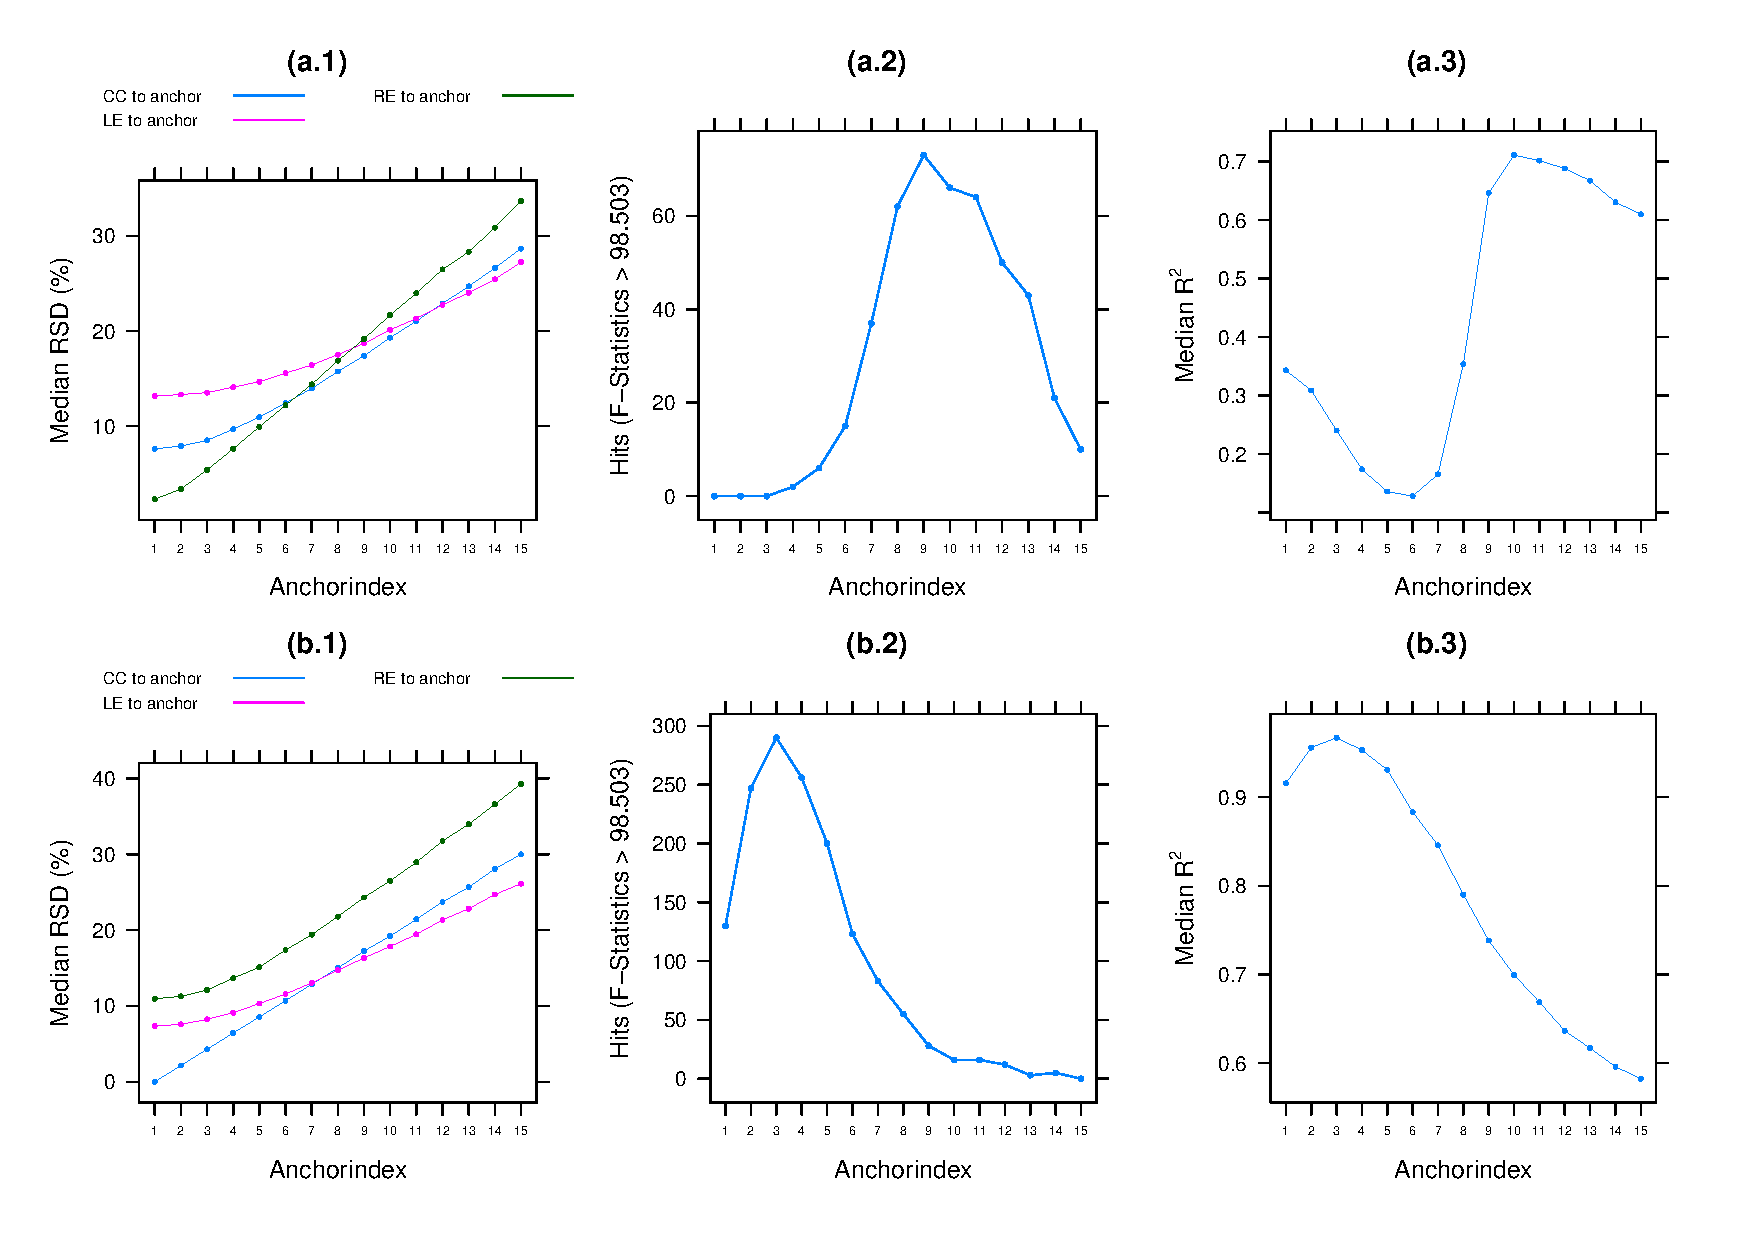
\includegraphics[scale=.48]{./plots/diag_allh.pdf}
\end{center}
\captionbelow[Diagnosticplot -- Example~\ref{subsubsec:a}]{This figure represents the the diagnosticplots for the example given in section~\ref{subsubsec:a}. It shows the outcome of the simulation testing for complex onset hypotheses.}
\label{pic:diag_exmp}
\end{figure}

\textbf{Figure (a/b.1):} change in stability pattern as a function of anchor variability. The first figure shows how the relative standard deviation of each interval measured in the simulated data changes as a function of the level of variability in the intervals.
This type of figure is used in~\textcite[][section 4.2]{Shaw2009} to show that stability patterns change under different conditions of overall variability.
In ParseEval, variability is infused in the simulated data through the standard deviation of the anchor point.
The size of the variability range considered by the model and the size of the stepwise increase in variability is specified in the function call.\par

\textbf{Figure (a/b.2):} line-plot of best-fitting variability level.
The second figure shows the total number of \enquote{Hits} achieved for each anchor. Each \enquote{Hit} indicates a simulation for the particular anchor, for which the OLS regression yielded F-statistics that were greater than 98.503\footnote{This particular value for the F-statistics marks a threshold of statistical significance}. The total number of \enquote{Hits} for a given anchor can be used as an indicator to assess how well the experimental data was fit by the simulated data. Anchor-indices with high numbers of \enquote{Hits} indicate variability-ranges where the simulated data matched the experimental data very well.\par

\textbf{Figure (a/b.3):} 
The third figure shows that median R-squared values across all simulations in relation to the anchorindex. In combining the information from Figure 2 and 3 this should further indicate which variability-ranges provided a match between the experimental and the simulated data.
\section{Quick start guide}
\label{sec:qsg}
This section skips any information and only represents example code. The data, code and diagnostic plots are taken from \textcite{Auris2013}.\\[1em]
\begin{lstlisting}
set.seed (2342) # make examples reproducible
parse_mina_smina <- parseEval(c1=c(82.637,9.332),c2=c(84.610,11.070),
c3=c(84.610,11.070),cipi12=c(71.186,15.798),cipi23=c(71.186,15.798),
voweld=307,types=2,RE_rsd=0.311,CC_rsd=0.263,LE_rsd=0.232)
\end{lstlisting}

Running the above code should produce an outcome looking similar to:
\begin{lstlisting}
Overall Quality of Modell-Performance	(Testing Dyads)
(Ratio of:	Total Number of Hits / Number of Simulations)
------------------------
Simple Modelling:	5.832				5832 / 1000

Complex Modelling:	0				0 / 1000
\end{lstlisting}

With corresponding diagnostic plots looking similar to the following figure.
\begin{figure}[htbp]
\begin{center}
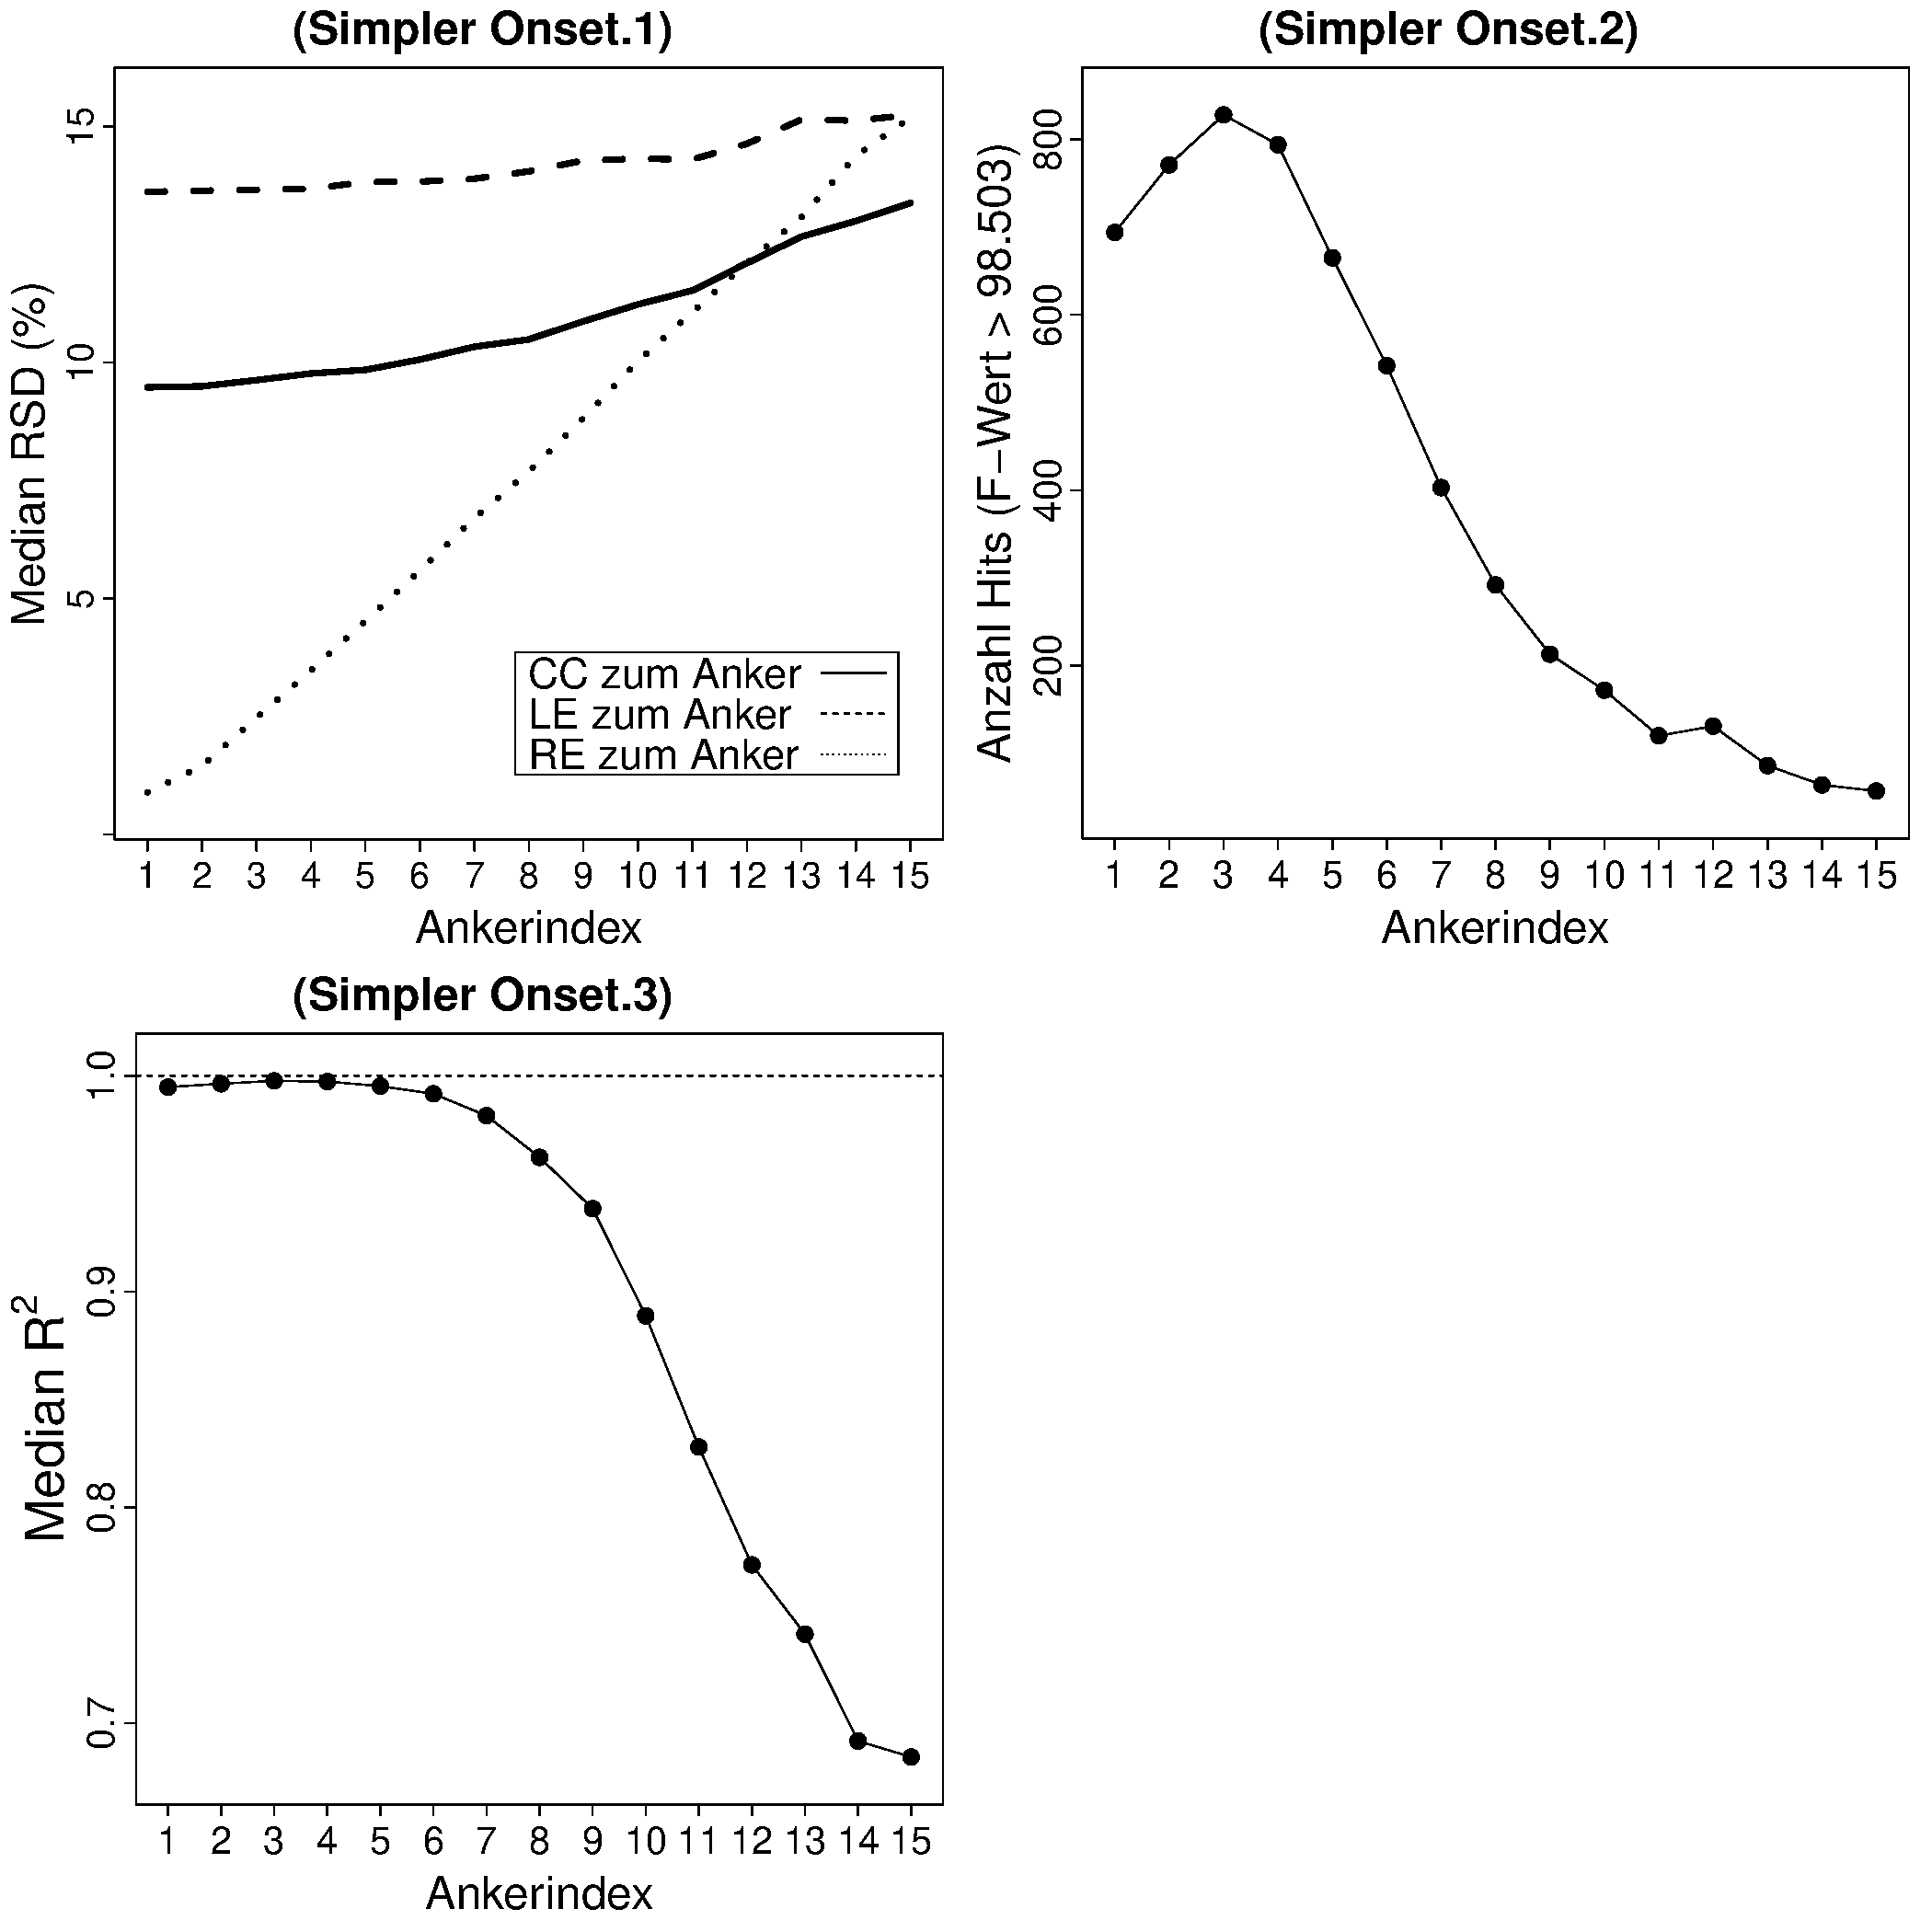
\includegraphics[scale=.4]{./plots/diag_simplex_parse_mina_smina5.pdf}
\end{center}
\captionbelow[Diagnosticplot -- Cluster /zm/]{Diagnosticplot generated from a succesfull parse. In particular (a.1-3) showing three plots that visualize the outcome of the parse corresponding to simple onset hypotheses. This parse was taken from analysing data of targetwords /mina/ -- /zmina/.}
\label{pic:diag_sm}
\end{figure}

\pagebreak
%references
\printbibliography[heading=bibintoc]
\pagebreak
%appendices
%\appendix
%\section*{Appendix}
%\addcontentsline{toc}{section}{Appendix}
\end{document}
